%\begin{savequote}[75mm]
%Nulla facilisi. In vel sem. Morbi id urna in diam dignissim feugiat. Proin molestie tortor eu velit. Aliquam erat volutpat. Nullam ultrices, diam tempus vulputate egestas, eros pede varius leo.
%\qauthor{Quoteauthor Lastname}
%\end{savequote}

\chapter{A Brief History of Neutrinos}

%\newthought{There's something to be said} for having a good opening line. Morbi commodo, ipsum sed pharetra gravida, orci  $x = 1/\alpha$ magna rhoncus neque, id pulvinar odio lorem non turpis \cite{Eigen1971, Knuth1968}. Nullam sit amet enim. Suspendisse id velit vitae ligula volutpat condimentum. Aliquam erat volutpat. Sed quis velit. Nulla facilisi. Nulla libero. Vivamus pharetra posuere sapien. Nam consectetuer. Sed aliquam, nunc eget euismod ullamcorper, lectus nunc ullamcorper orci, fermentum bibendum enim nibh eget ipsum. Donec porttitor ligula eu dolor. Maecenas vitae nulla consequat libero cursus venenatis. Nam magna enim, accumsan eu, blandit sed, blandit a, eros.
%$$\zeta = \frac{1039}{\pi}$$

\section{Introduction}

The neutrino was first postulated by Wolfgang Pauli as a possible explanation for the continuous spectrum of electrons emitted from nuclear $\beta$ decay \cite{ref:Pauli}. This decay was originally thought to be the emission of an electron from an atom, resulting in a different nucleus, via the process,

\beq
N \rightarrow N' + e
\label{eq:BetaWrong}
\eeq

\n where $N$ and $N'$ are the parent and daughter nuclei, respectively. In a two body decay such as this, the momenta and energies of the outgoing particles are exactly constrained. Pauli's new particle explained the continuous spectrum of electron energy via a modified decay process:

\beq
N \rightarrow N' + e + \nu
\label{eq:BetaRight}
\eeq

\n where $\nu$ is the outgoing neutral particle. Pauli's original proposal called the new particle the neutron, but this name was later used to name the massive neutral nucleon discovered by Chadwick in 1932 \cite{ref:Chadwick}. Three years after Pauli's idea, Fermi proposed a model for nuclear $\beta$ decay that included the new particle, which he coined the neutrino, or little neutral one \cite{ref:Fermi}.

\section{First Detection of Neutrinos}

Twenty years passed from Fermi's model proposal before neutrinos were discovered experimentally. Fred Reines and Clyde Cowan made the discovery by placing a detector near a nuclear reactor as a source of neutrinos and observing inverse $\beta$ decay \cite{ref:1953, ref:1956}. The neutrinos observed were anti-electron neutrinos, thus the following was the observed process.

\beq
p + \anue \rightarrow n + e^{+}
\label{eq:BetaInv}
\eeq

\n Reines earned the Nobel Prize in Physics in 1995 for the detection of the neutrino.

In 1962, the muon neutrino was discovered at Brookhaven National Laboratory using the first neutrino beam \cite{ref:BNL} in a scheme still used in neutrino experiments today. The beam was generated by colliding protons with a target, producing pions that decayed into muons and muon neutrinos. The resultant beam then passed through thick steel, absorbing everything but the neutrinos. Leon Lederman, Melvin Schwartz, and Jack Steinberger won the Nobel Prize in Physics in 1988 for the discovery of the muon neutrino.

The last generation of neutrino, the tau neutrino, was discovered at Fermilab by the DONUT collaboration in 2000 \cite{ref:DONUT}.

\section{Evidence of Neutrino Oscillations}

Pontecorvo first postulated neutrino oscillations between neutrinos and anti-neutrinos, analogous to $K^0/\bar{K}^0$ oscillations, in 1957 \cite{ref:Pontecorvo1}. Nothing came of the proposal immediately, but the idea was later revived and modified to solve the solar neutrino problem. The physics community initially viewed neutrino oscillations with skepticism and believed the experiments to be flawed, but over time oscillations have become an unmistakable and accepted phenomenon.

The solar neutrino problem was born from a large discrepancy between the theoretical and observed number of neutrinos produced by the sun. Neutrinos were used as a study for solar models because photons take a thousand years to escape the dense nuclear plasma to the surface of the sun, but neutrinos are unimpeded. The models, which have been confirmed today, describe a somewhat complicated chain of nuclear reactions, many of which produce neutrinos. Each individual process contributes a neutrinos in a different energy spectrum, but all of the neutrinos are created as electron neutrinos.

The experimental observations and theoretical predictions were both published in 1968. Ray Davis designed an experiment underground in the South Dakota Homestake mine consisting of a tank of an ultra pure chlorine cleaning solution capable of neutrino capture via the process

\beq
\nue +\mbox{ \textsuperscript{37}Cl }\rightarrow\mbox{ \textsuperscript{37}Ar }+ e^{-}
\label{eq:DavisExp}
\eeq

\n The argon atoms could be collected and counted for a direct measurement of the neutrino flux \cite{ref:Davis}. Meanwhile, John Bahcall precisely calculated the expected neutrino flux \cite{ref:Bahcall}, and the observed rate was found to be about one third of the predicted rate. Pontecorvo revived his theory with the modification of allowing $\nue$ to $\numu$ oscillations \cite{ref:Pontecorvo2}, but the idea was still not taken seriously and it was another 20 years before the solar neutrino problem was confirmed. 

Beginning in 1989, multiple experiments with different methodologies confirmed the solar neutrino problem. Kamiokande, a water Cherenkov detector, measured a rate deficit in 1989 \cite{ref:Kamiokande}. Two experiments measured solar neutrinos via the reaction

\beq
\nue + \mbox{ \textsuperscript{71}Ga } \rightarrow \mbox{ \textsuperscript{71}Ge } + e^{-}
\label{eq:GaExp}
\eeq

\n and measured a similar deficit, SAGE in 1991 \cite{ref:SAGE} and GALLEX in 1992 \cite{ref:GALLEX}. With results from three different experimental methods all showing similar rate deficits, the solar neutrino problem could no longer be relegated to an experimental error.

Evidence soon emerged for oscillations with atmospheric neutrinos as well. These neutrinos are produced when cosmic rays collide with particles in the atmosphere and decay, predominantly via the following channels.

\beqa
\pi^{+/-} & \rightarrow & \mu^{+/-} + \numu/\anumu \nonumber \\
\mu^{+/-} & \rightarrow & e^{+/-} + \nue/\anue + \anumu/\numu
\label{eq:AtmNu}
\eeqa

\n Thus, the expected ratio of muon family neutrinos to muon family neutrinos was expected to be 2. Kamiokande measured this ratio in 1992 and found the ratio to be much closer to 1 \cite{ref:KamioAtm}. Furthermore, the ratio seemed to be dependent on zenith angle, with the measurement being nearly 2 for neutrinos coming from directly overhead, and dropping as the angle increased. Super-Kamiokande (or Super-K), the successor to Kamiokande, improved upon this measurement in 1998 \cite{ref:SuperKAtm}, providing the most definitive evidence of neutrino oscillations to that point.

A resolution to the solar neutrino problem did not have to wait much longer with detector technologies capable of discerning different neutrino interaction types. SNO was designed as a heavy water (D\textsubscript{2}O) Cherenkov detector experiment to be sensitive to both the flux of electron neutrinos and the flux of all neutrinos. In 2002, it released results for these measurements, finding what was then the expected deficit in electron neutrino flux, but a total flux consistent with the standard solar model, see Fig.~\ref{fig:SNO} \cite{ref:SNO02}. With this result, neutrino oscillations were confirmed, and subsequent experiments now measure oscillation parameters with precision.

\begin{figure}
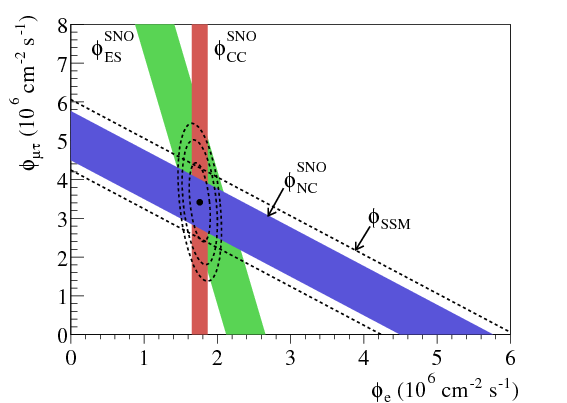
\includegraphics[width=\textwidth]{figures/SNOResult.png}
\caption[SNO Result]{The measurement of different event rates at SNO \cite{ref:SNO02}. The red band represents $\nue$ CC interactions with the deuterium neutron, an interaction only sensitive to electron neutrinos. The blue band represents neutral current scattering off of the deuterium nucleus, an interaction sensitive to the total neutrino flux. The green band represents elastic scattering of the neutrino off the deuterium electron, an interaction sensitive to all neutrino flavors, but not completely independent of neutrino flavor. The dashed straight lines represent the flux prediction by the standard solar model. The point represents the best fit for the flux of electron neutrinos and the flux for the combined muon and tau neutrinos.
\label{fig:SNO}}
\end{figure}

\section{Possible Evidence of Sterile Neutrinos}

There exists some evidence of more than three neutrinos, but the number of active neutrinos is constrained by measurements of the width of the Z boson. LEP has measured the number of active neutrinos to be $2.984 \pm 0.008$ \cite{ref:LEP}, so the discoveries of the $\nue$, $\numu$, and $\nutau$ leave no room for new active neutrinos. (Strictly speaking, there could be other active neutrinos if they had mass greater than half the mass of the Z boson so the Z could not decay to them, but the evidence that does exist suggests a mass splitting from the other neutrino states much smaller than this.)

% For an example of a full page figure, see Fig.~\ref{fig:myFullPageFigure}.

%\texttt{This is a line of code.}

%\begin{figure}
%\includegraphics[width=\textwidth]{figures/fig1}
%\caption[Short figure name.]{This is a figure that floats inline and here is its caption.
%\label{fig:myInlineFigure}}
%\end{figure}

%% Requires fltpage2 package
%%
% \begin{FPfigure}
% \includegraphics[width=\textwidth]{figures/fullpage}
% \caption[Short figure name.]{This is a full page figure using the FPfigure command. It takes up the whole page and the caption appears on the preceding page. Its useful for large figures. Harvard's rules about full page figures are tricky, but you don't have to worry about it because we took care of it for you. For example, the full figure is supposed to have a title in the same style as the caption but without the actual caption. The caption is supposed to appear alone on the preceding page with no other text. You do't have to worry about any of that. We have modified the fltpage package to make it work. This is a lengthy caption and it clearly would not fit on the same page as the figure. Note that you should only use the FPfigure command in instances where the figure really is too large. If the figure is small enough to fit by the caption than it does not produce the desired effect. Good luck with your thesis. I have to keep writing this to make the caption really long. LaTex is a lot of fun. You will enjoy working with it. Good luck on your post doctoral life! I am looking forward to mine. \label{fig:myFullPageFigure}}
% \end{FPfigure}
% \afterpage{\clearpage}
